%   Filename    : chapter_4.tex 
\chapter{System Architecture and Model Evaluation}
\section{System Architecture}
Using the tools mentioned in Section~\ref{sec:devtools}, our system can be visualized as shown in Figure \ref{fig:architecture}: 
\begin{figure}[h] % 'h' places the figure approximately here in the text
	\centering
	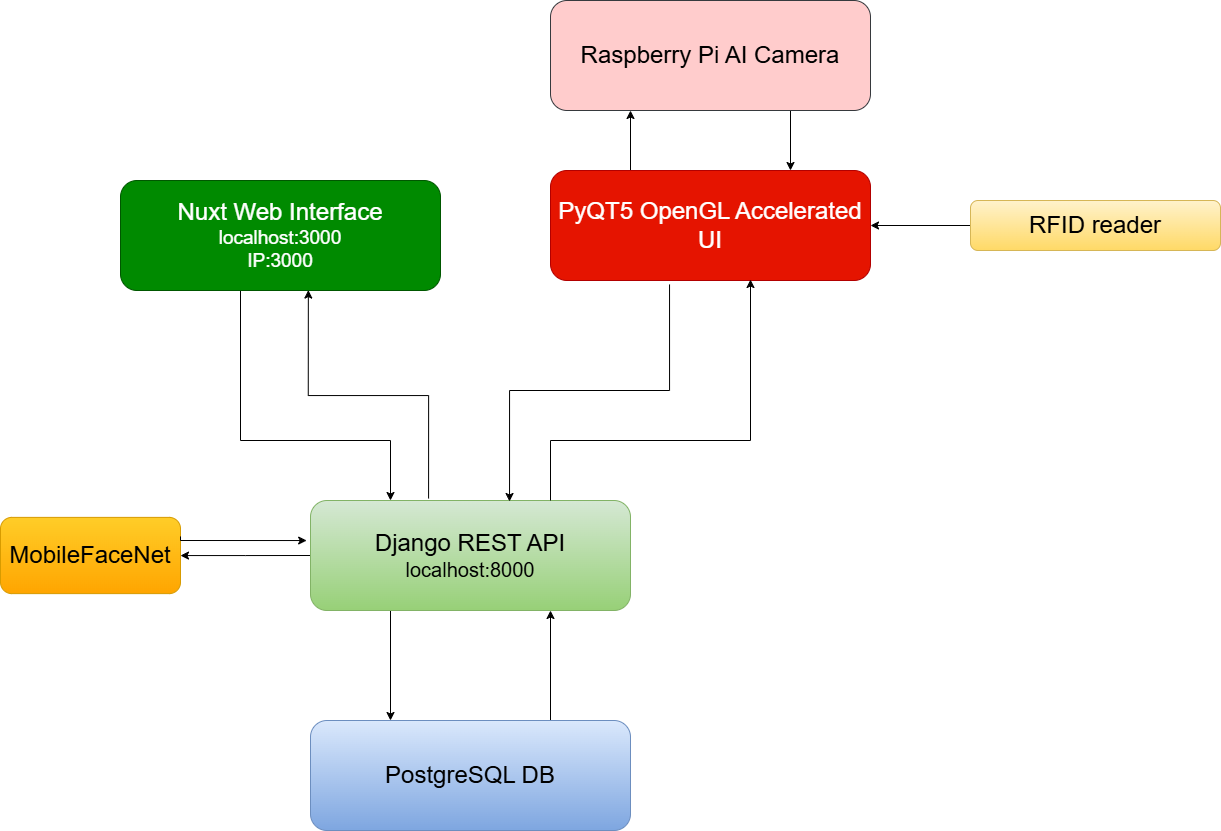
\includegraphics[width=0.55\textwidth]{figures/chapter4/architecture_new.png} % Adjust width as needed
	\caption{System Architecture}
	\label{fig:architecture}
\end{figure}
All of the software and services are running in the Raspeberry Pi 5. We have no online dependencies except the Hero icons which are MIT licensed and free to use.

\section{Process Diagram}

\subsection{Student Registration Process}
Students must register their facial ID to enable attendance verification. This registration process only captures one facial image, which will be used to identify the student during attendance tracking. It also takes all relevant info about the student, reflecting the fields given by the generated class list of CRS. It will be handled by Nuxt at endpoint: \url{http://raspberry_ip:3000/public/register. }
\begin{figure}[h] % 'h' places the figure approximately here in the text
	\centering
	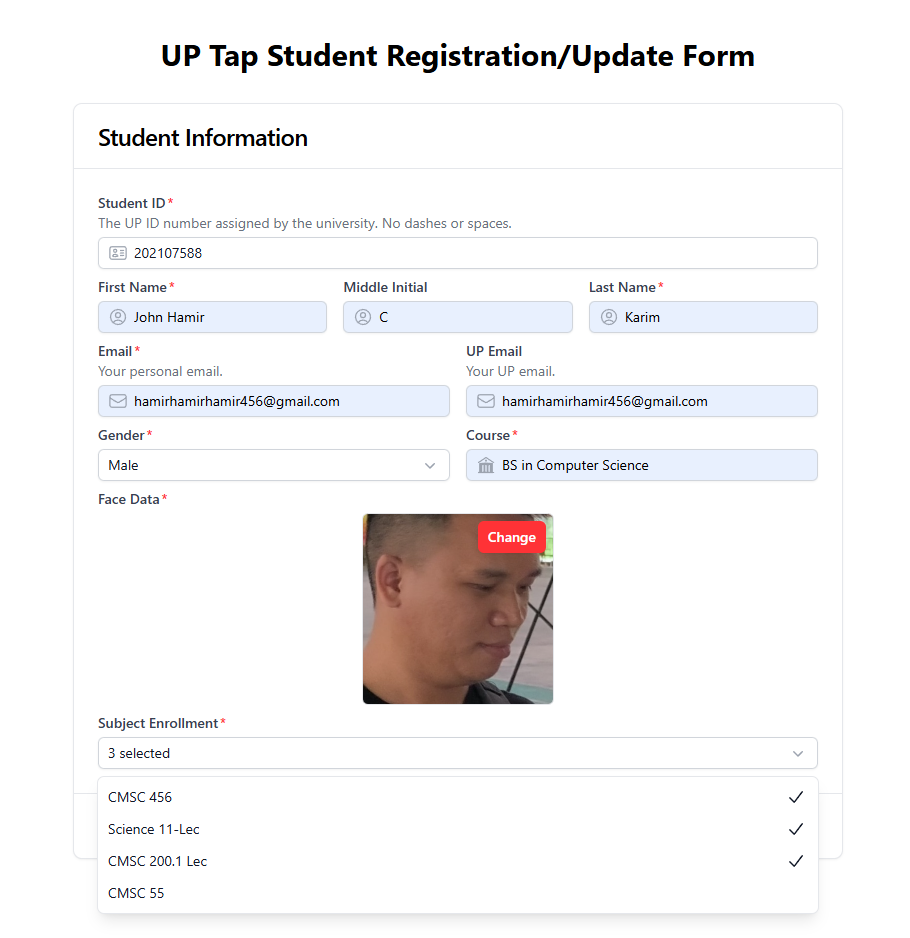
\includegraphics[width=0.8\textwidth]{figures/chapter4/student_form_pc.png} % Adjust width as needed
	\caption{Form in desktop client. Face data defaults to file picker. It will still check for faces in the image.}
	\label{fig:student_form_pc}
\end{figure}
\clearpage

\begin{figure}[h] % 'h' places the figure approximately here in the text
	\centering
	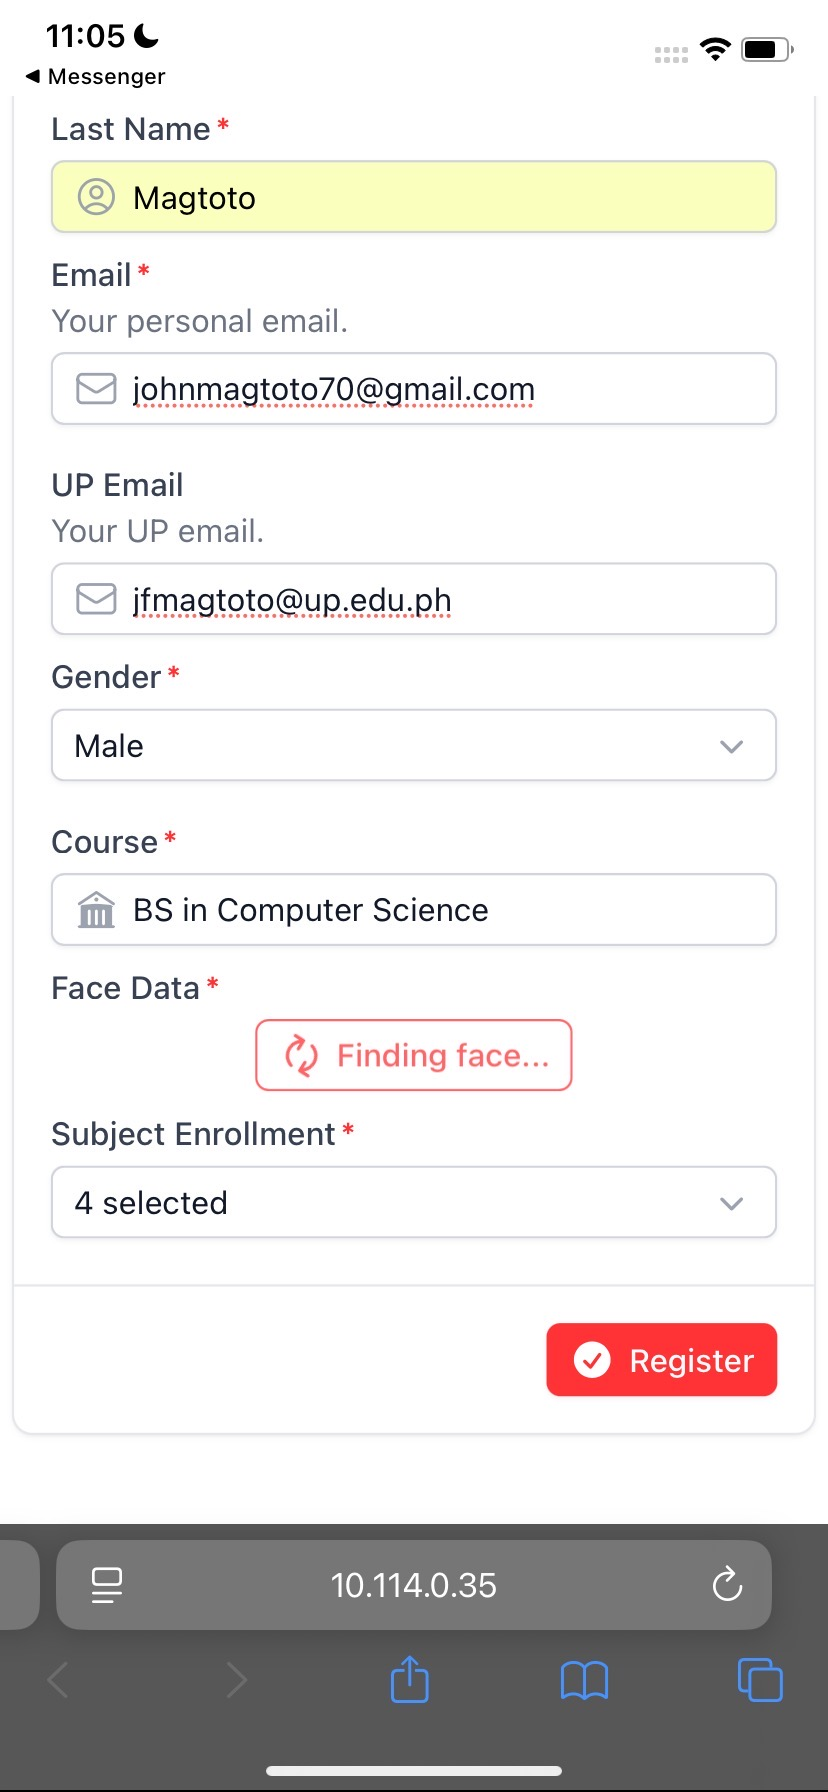
\includegraphics[width=0.5\textwidth]{figures/chapter4/student_form_mobile.jpg} % Adjust width as needed
	\caption{Form in mobile devices. Face data will use the native camera instead. It will then detect faces from the image provided.}
	\label{fig:student_form_mobile}
\end{figure}
\clearpage
\begin{figure}[h] % 'h' places the figure approximately here in the text
	\centering
	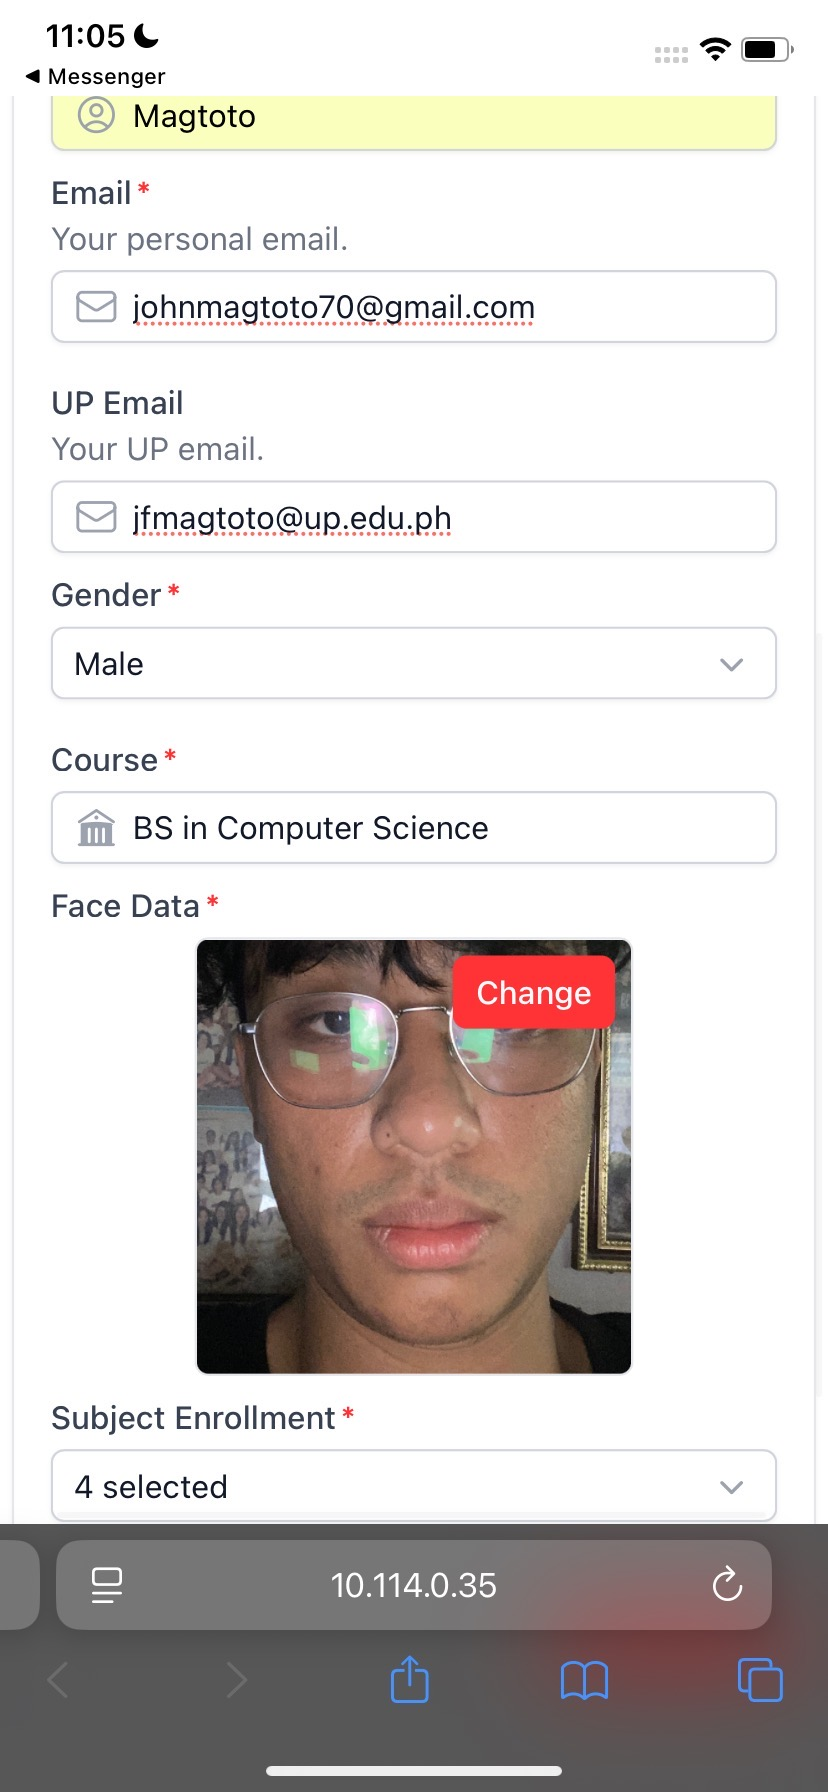
\includegraphics[width=0.5\textwidth]{figures/chapter4/student_form_mobile_preview.jpg} % Adjust width as needed
	\caption{Face data preview when face is detected. Otherwise show an alert window for image retake.}
	\label{fig:student_form_mobile_preview}
\end{figure}
\clearpage
\subsection{Time In Process}
Time in process includes a check if the student already has time in records. First step in this is the student tapping the ID to the RFID sensor and trigger the photo capture to check the face.
\begin{figure}[h] % 'h' places the figure approximately here in the text
	\centering
	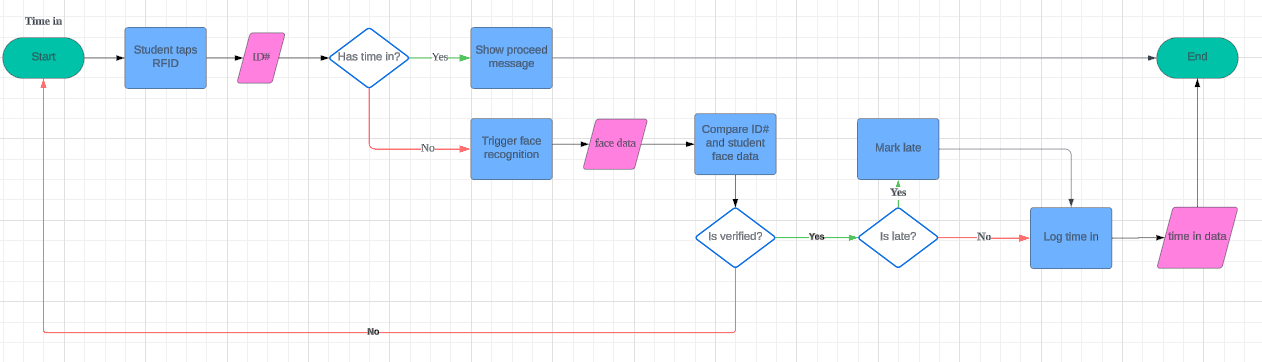
\includegraphics[width=1.0\textwidth]{figures/chapter4/timein.png} % Adjust width as needed
	\caption{Time in}
	\label{fig:timein}
\end{figure}

\clearpage
\subsection{Time Out Process}
\begin{figure}[h] % 'h' places the figure approximately here in the text
	\centering
	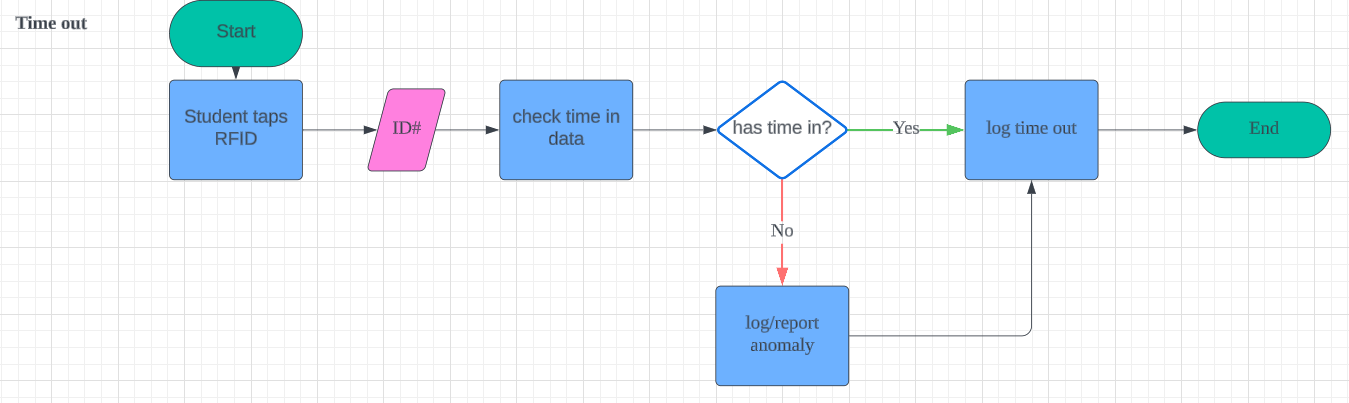
\includegraphics[width=1.0\textwidth]{figures/chapter4/timeout.png} % Adjust width as needed
	\caption{Time Out}
	\label{fig:timeout}
\end{figure}

\subsection{Attendance Record Export Process}
The faculty members are allowed to export their attendance records into a CSV/PDF file in order to have better access and record keeping. In addition to that, this feature can be useful for further analysis, for data backup purposes, or if they want to integrate it into another academic system. 
\begin{figure}[h] % 'h' places the figure approximately here in the text
	\centering
	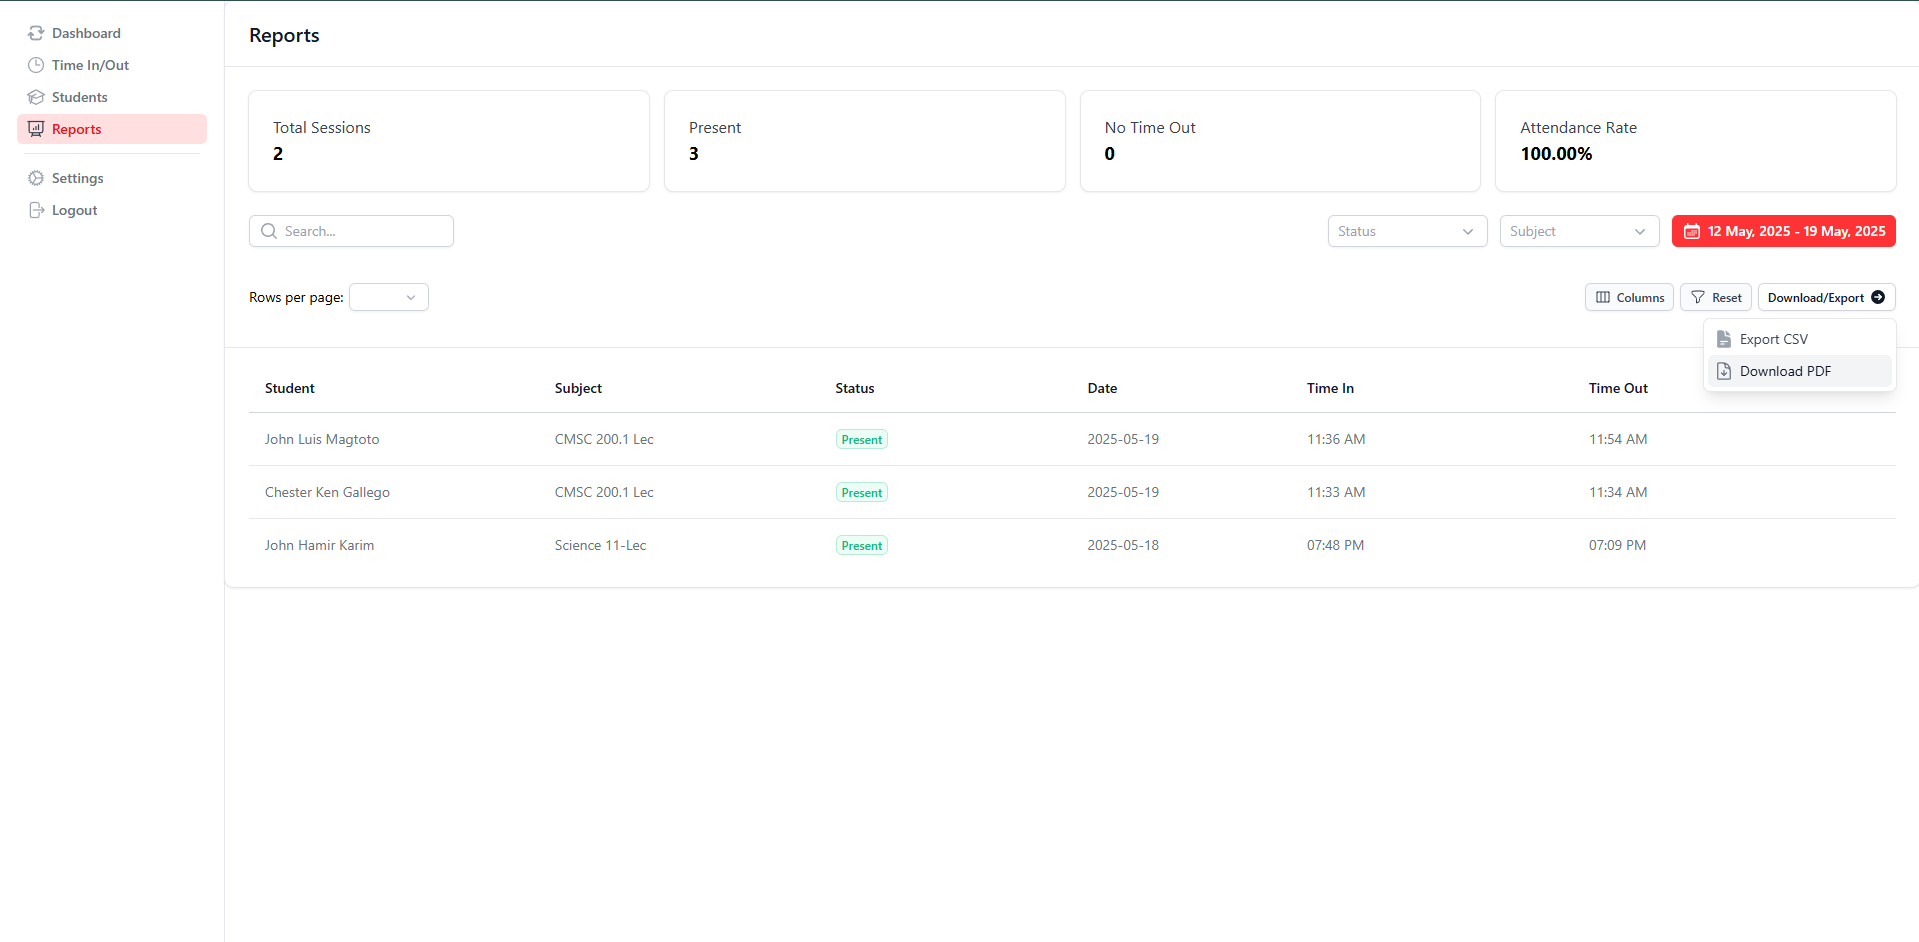
\includegraphics[width=1.0\textwidth]{figures/chapter4/att_ui.png} % Adjust width as needed
	\caption{Reports page}
	\label{fig:att_ui}
\end{figure}
\begin{figure}[h] % 'h' places the figure approximately here in the text
	\centering
	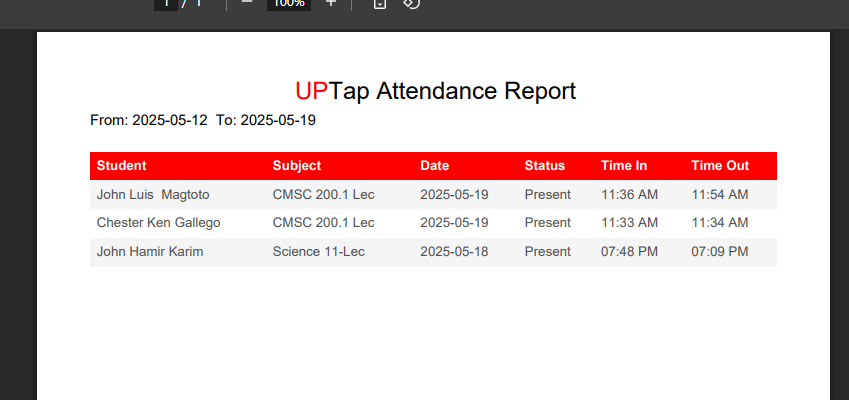
\includegraphics[width=1.0\textwidth]{figures/chapter4/att_report.png} % Adjust width as needed
	\caption{Report PDF}
	\label{fig:att_report}
\end{figure}
\clearpage
\section{Django Backend}
\subsection{Models}
Django Model class maps to SQL tables. For example, a Student table will have the following columns which maps to Student Model class' attributes like in Figure \ref{fig:models}: 

\begin{figure}[h] % 'h' places the figure approximately here in the text
	\centering
	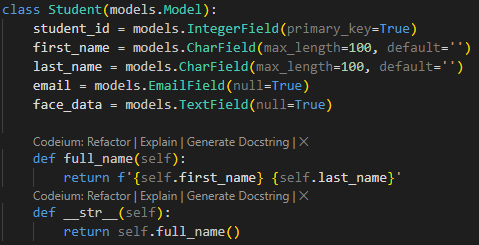
\includegraphics[width=0.8\textwidth]{figures/chapter4/models.png} % Adjust width as needed
	\caption{Student model}
	\label{fig:models}
\end{figure}

SQL equivalent would be:
\begin{verbatim}
	CREATE TABLE Student (
	student_id INTEGER PRIMARY KEY,
	first_name VARCHAR(100) NOT NULL DEFAULT '',
	last_name VARCHAR(100) NOT NULL DEFAULT '',
	email VARCHAR(254),
	face_data TEXT,
	CONSTRAINT unique_email UNIQUE (email)
	);
\end{verbatim}
\subsection{Database Table}
The database tables are automatically generated using django-extensions module. It reads all the Model classes in our Django project and generates the connections between tables.
\begin{figure}[h] % 'h' places the figure approximately here in the text
	\centering
	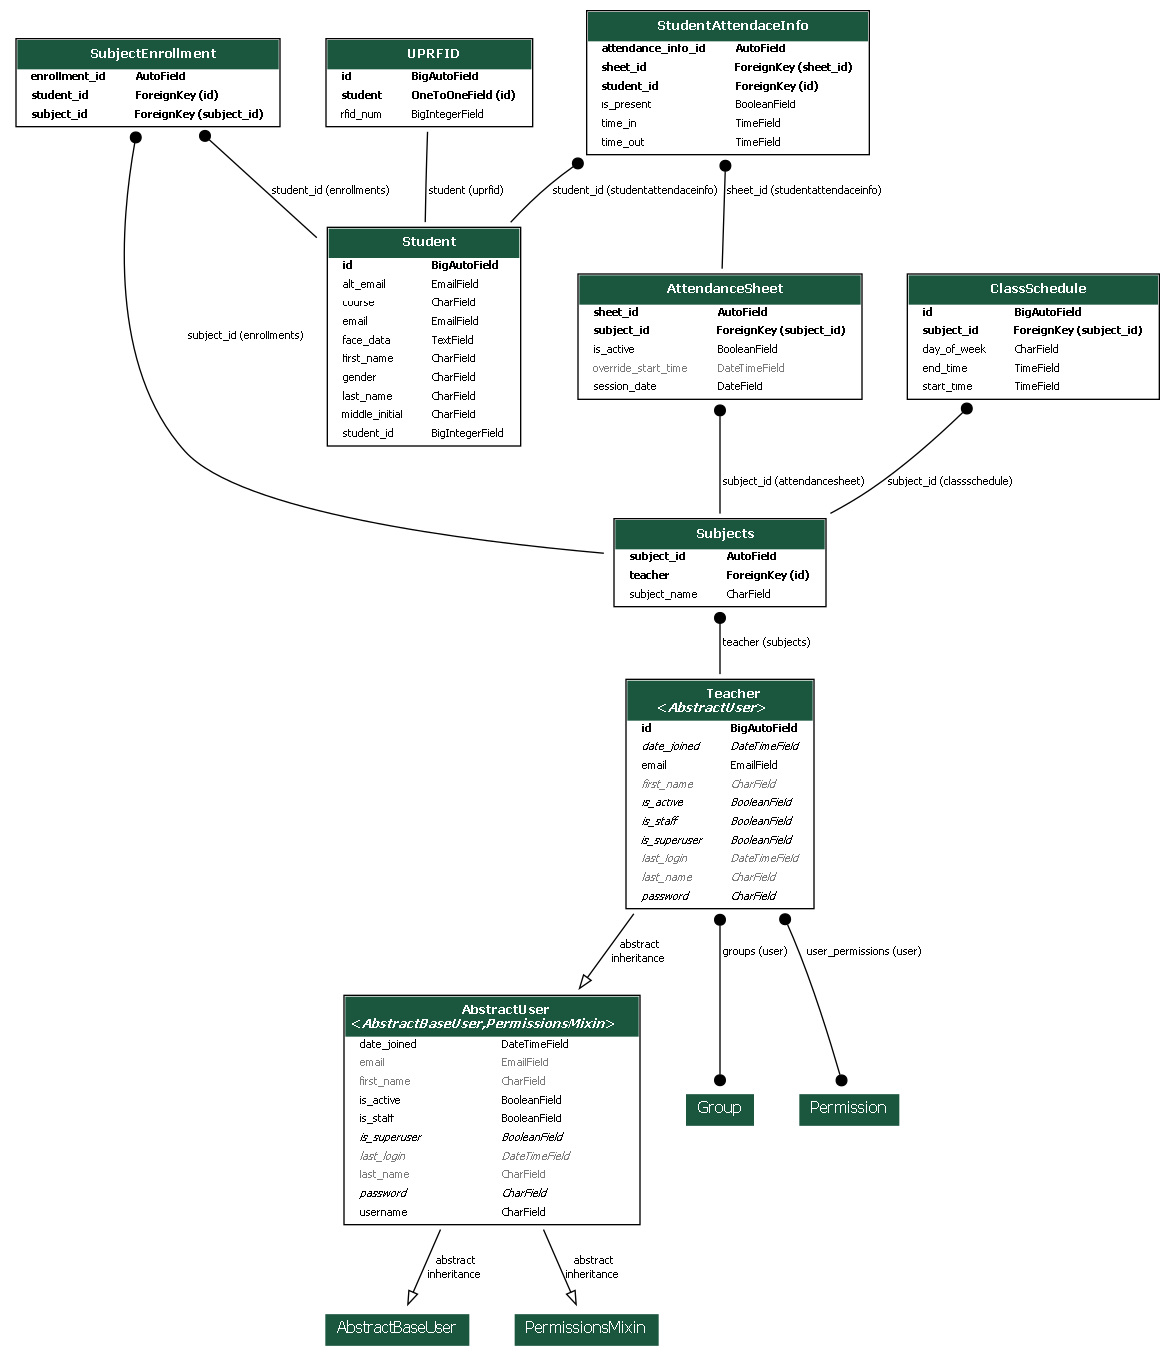
\includegraphics[width=0.8\textwidth]{figures/chapter4/db_tables.png} % Adjust width as needed
	\caption{System Architecture}
	\label{fig:db_tables}
\end{figure}	

\subsection{REST API by Django Ninja}
Figure~\ref{fig:api} is the automatic OpenAPI compliant documentation provided by Django Ninja. It contains all endpoints we can use to query data from the database. All endpoints are protected using HTTP Bearer token authentication.
\begin{figure}[h] % 'h' places the figure approximately here in the text
	\centering
	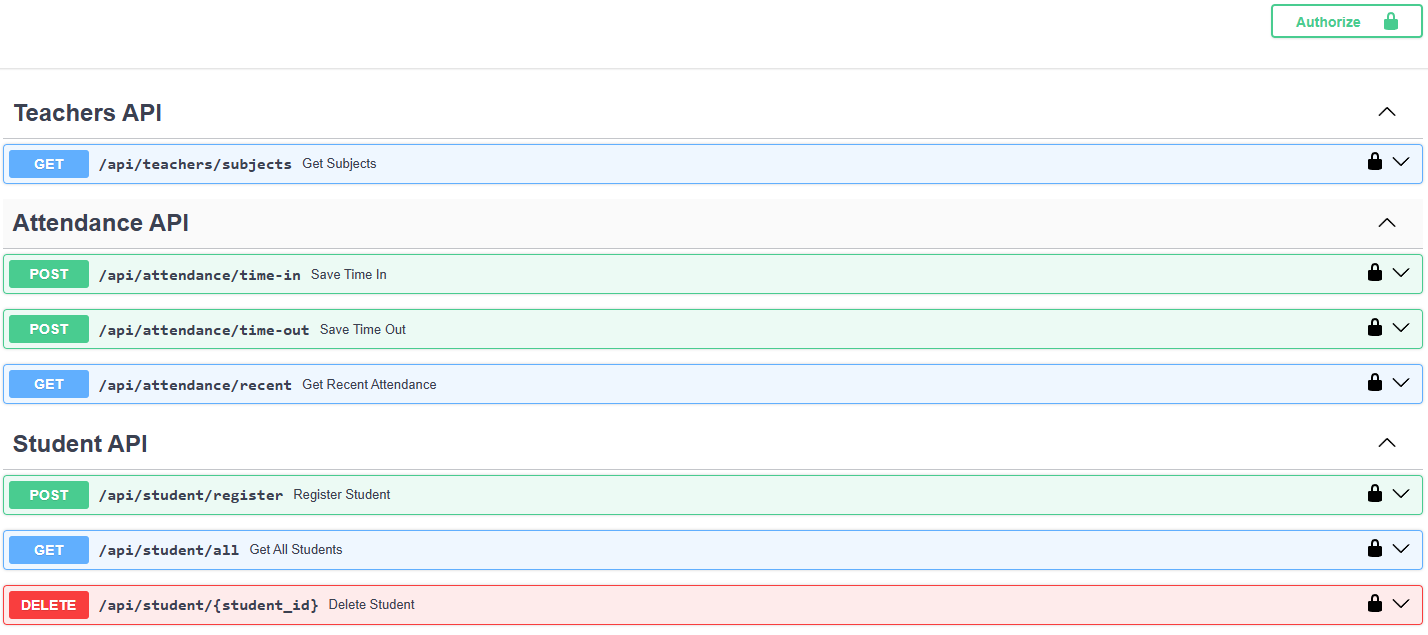
\includegraphics[width=1\textwidth]{figures/chapter4/api.png} % Adjust width as needed
	\caption{API Documentation}
	\label{fig:api}
\end{figure}

\subsection{Admin panel by Django}
Figure~\ref{fig:admin} is the Django administration page only accessible to a superuser account. This is where most of the backend maintanance work happens. It contains all the data inside the database allow full control over them. It also contains every authentication tokens used by each teacher account.
\begin{figure}[h] % 'h' places the figure approximately here in the text
	\centering
	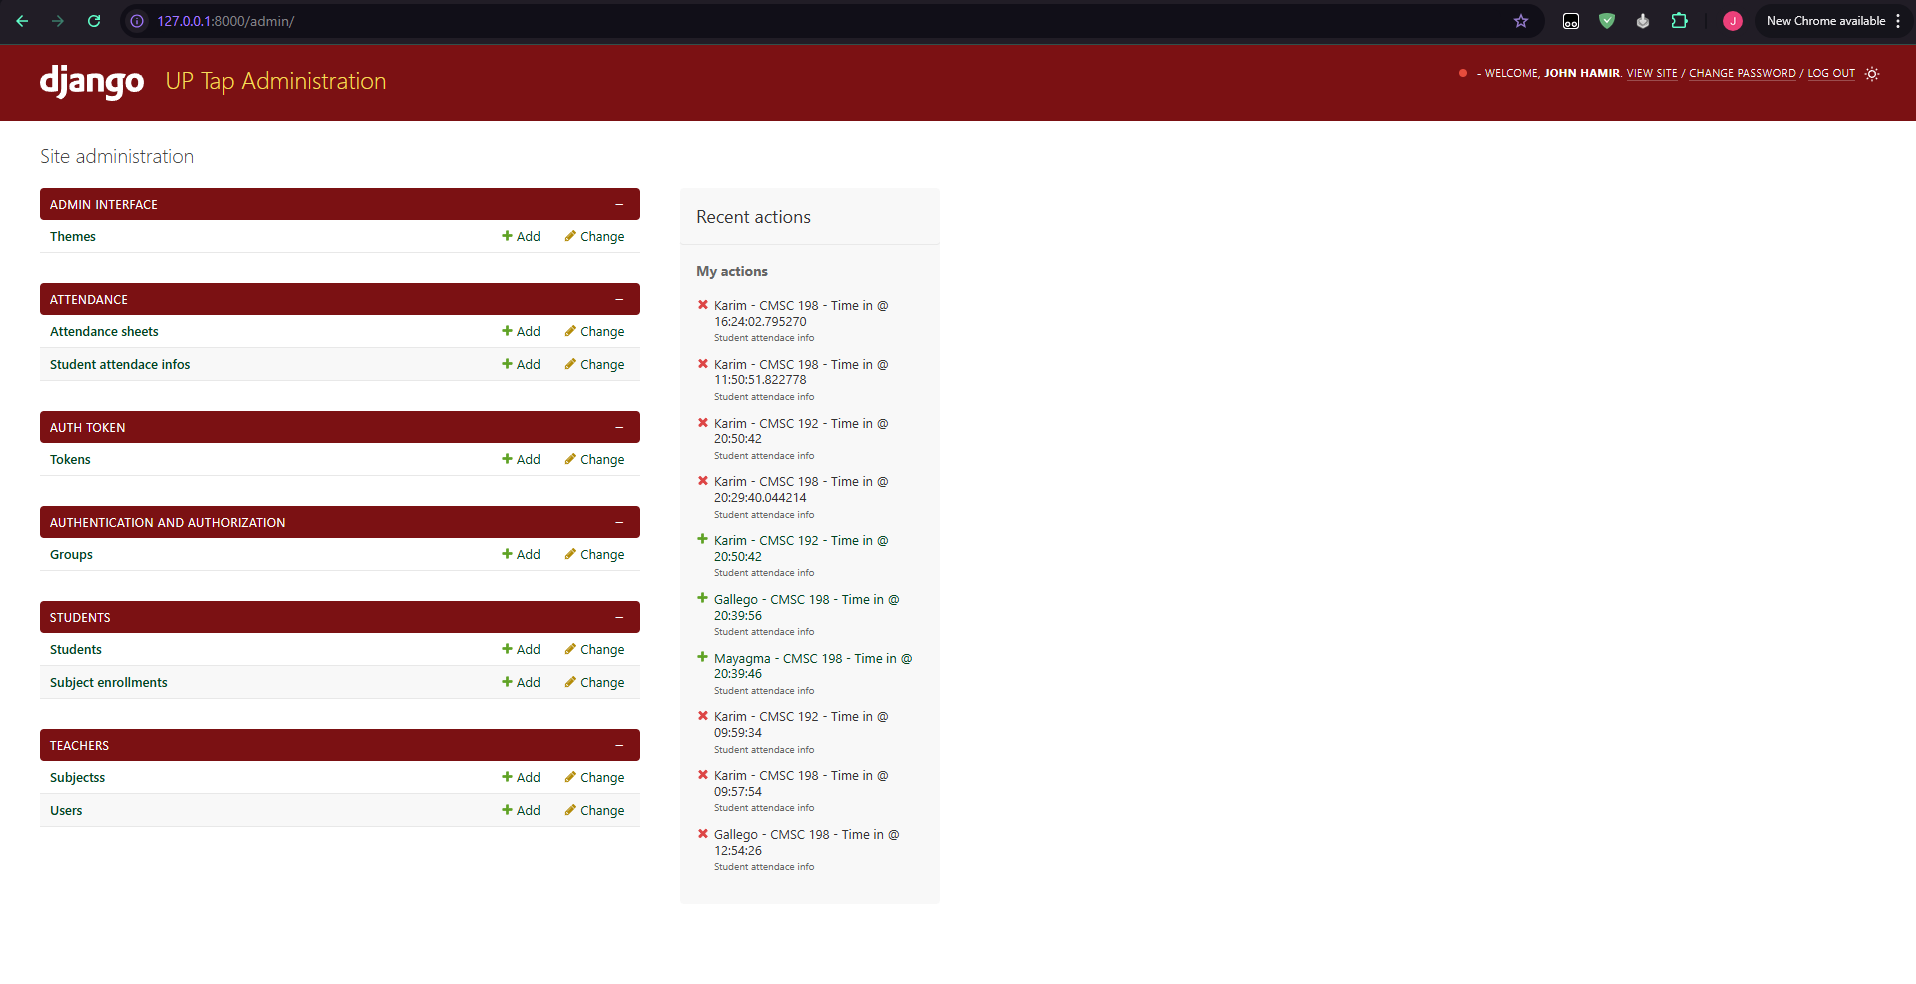
\includegraphics[width=1\textwidth]{figures/chapter4/admin.png} % Adjust width as needed
	\caption{Django Administration}
	\label{fig:admin}
\end{figure}

\section{Nuxt Frontend}
The Nuxt web interface functions as the main UI with out system. It handles faculty onboarding and CSV imports of their class list from the CRS. It also has student management system for the basic CRUD operations for students' information.
\subsection{Faculty Onboarding}
The faculty must register using their email and personal details to use the system. We can verify the authenticity of the email by sending them a link that activates the newly created account. After the registration process, they can now log in and use the system.
\begin{figure}[h] % 'h' places the figure approximately here in the text
	\centering
	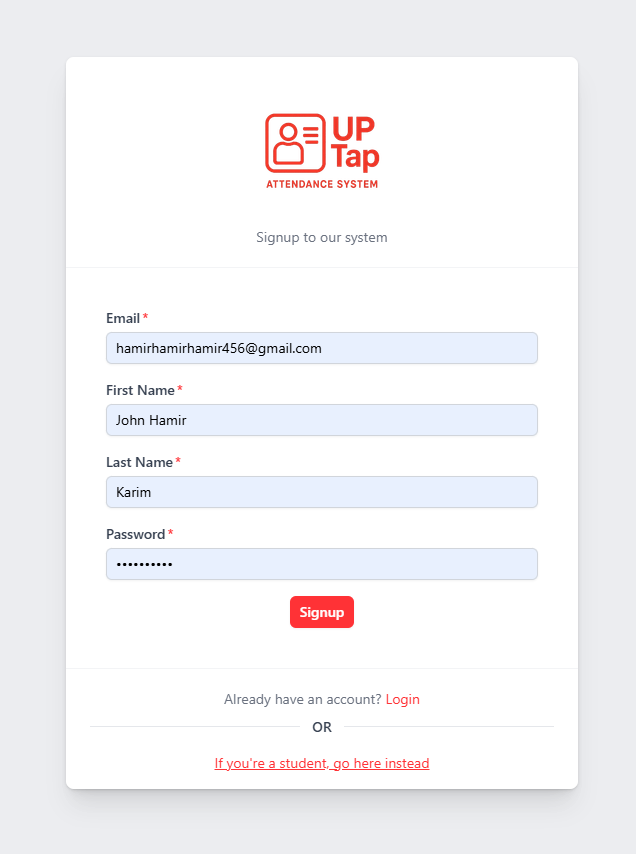
\includegraphics[width=0.8\textwidth]{figures/chapter4/faculty_signup.png} % Adjust width as needed
	\caption{Faculty Signup using email, first name, and last name}
	\label{fig:faculty_signup}
\end{figure}
\clearpage
\begin{figure}[h] % 'h' places the figure approximately here in the text
	\centering
	
\includegraphics[width=0.8\textwidth]{figures/chapter4/faculty_signup_info.png} % Adjust width as needed
	\caption{Notice after new signup}
	\label{fig:faculty_signup_info}
\end{figure}
\begin{figure}[h] % 'h' places the figure approximately here in the text
	\centering
	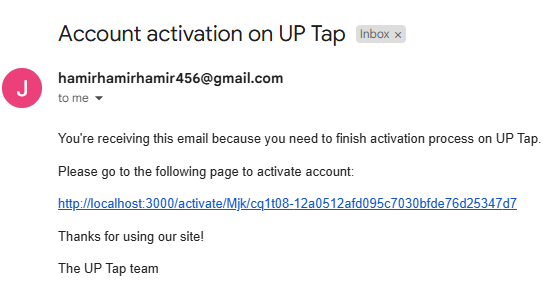
\includegraphics[width=0.8\textwidth]{figures/chapter4/faculty_signup_email.png} % Adjust width as needed
	\caption{Email containing the link for activation. Activation must be done on the same device.}
	\label{fig:faculty_signup_email}
\end{figure}
\begin{figure}[h] % 'h' places the figure approximately here in the text
	\centering
	
\includegraphics[width=0.8\textwidth]{figures/chapter4/faculty_activation.png} % Adjust width as needed
	\caption{Activating account on the link provided.}
	\label{fig:faculty_activation}
\end{figure}
\begin{figure}[h] % 'h' places the figure approximately here in the text
	\centering
	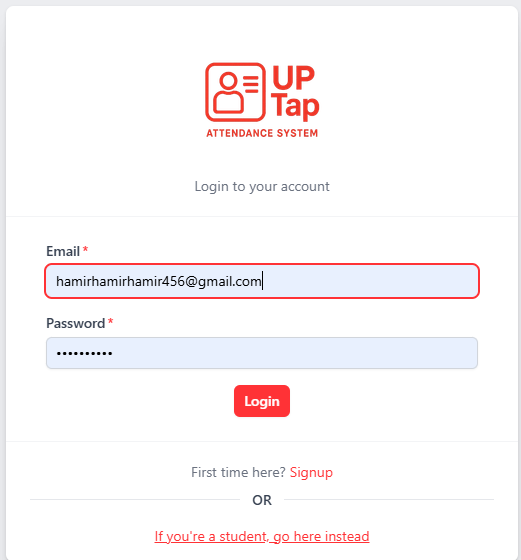
\includegraphics[width=0.8\textwidth]{figures/chapter4/faculty_login.png} % Adjust width as needed
	\caption{We can now login after opening the link.}
	\label{fig:faculty_login}
\end{figure}
\clearpage

\subsection{Subject CRUD Operations}
Each faculty is able to create subjects on their own, but it should not conflict with the time schedules of other faculty members. The system will warn for such conflicts. The modal for subject creation will provide a view of available time slots not taken by other subjects.
\begin{figure}[h] % 'h' places the figure approximately here in the text
	\centering
	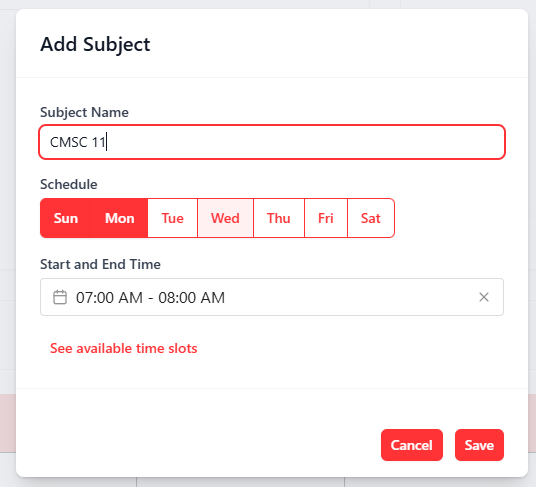
\includegraphics[width=0.8\textwidth]{figures/chapter4/subject_add.png} % Adjust width as needed
	\caption{Adding new subjects}
	\label{fig:subject_add}
\end{figure}
\begin{figure}[h] % 'h' places the figure approximately here in the text
	\centering
	
\includegraphics[width=0.8\textwidth]{figures/chapter4/subject_add_success.png} % Adjust width as needed
	\caption{Success}
	\label{fig:subject_add_success}
\end{figure}
\clearpage
\begin{figure}[h] % 'h' places the figure approximately here in the text
	\centering
	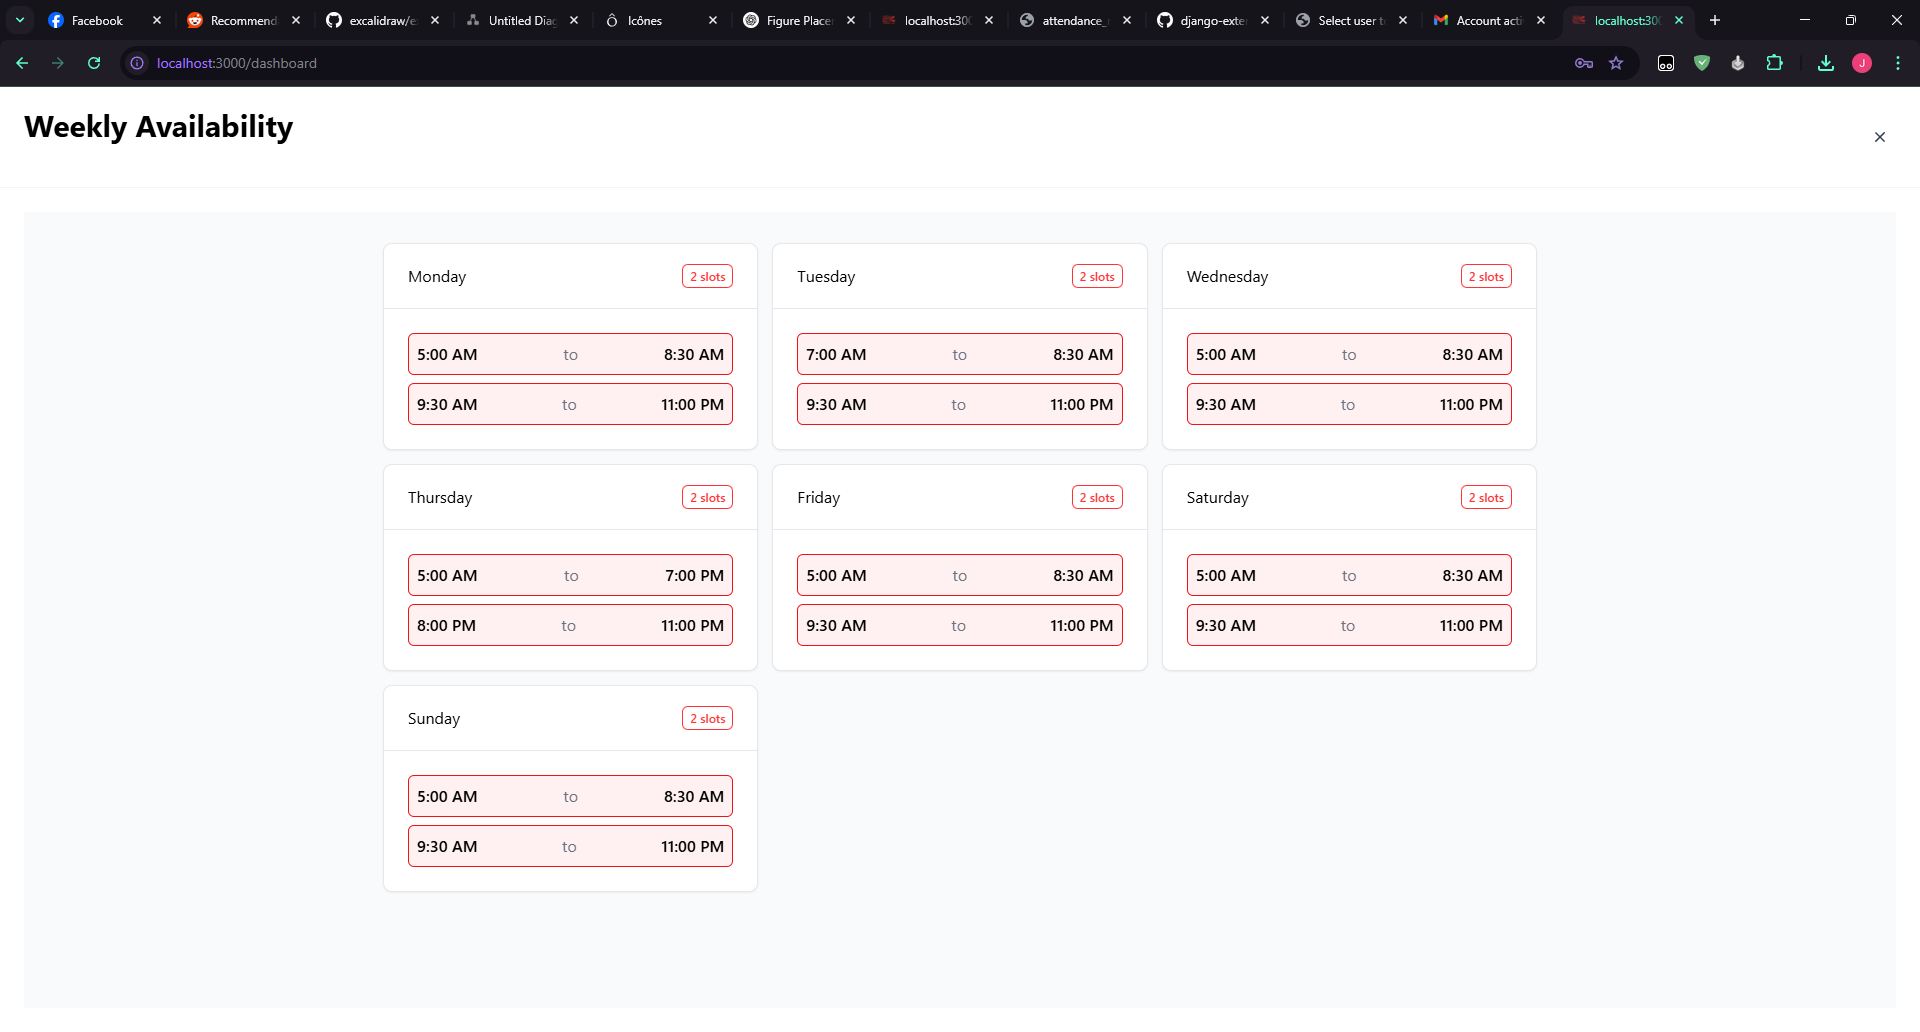
\includegraphics[width=0.8\textwidth]{figures/chapter4/subject_availability.png} % Adjust width as needed
	\caption{Available slots}
	\label{fig:subject_availability}
\end{figure}
\begin{figure}[h] % 'h' places the figure approximately here in the text
	\centering
	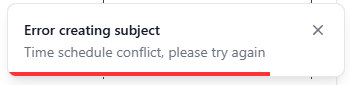
\includegraphics[width=0.8\textwidth]{figures/chapter4/subject_add_error.png} % Adjust width as needed
	\caption{Error due to time conflict}
	\label{fig:subject_add_error}
\end{figure}
\subsection{Faculty CSV Import Process}
After adding subjects, we can now import class list in CSV format. The faculty members can upload a CSV file containing the students' details. The system parses the CSV file and stores the extracted data in the database. The data uploaded is validated to avoid any duplicate or wrong entries. The backend populates/updates the Student table with the data and creates entries in the SubjectEnrollment table to tie each Student to a Subject. See Figure \ref{fig:faculty_import}
\begin{figure}[h] % 'h' places the figure approximately here in the text
	\centering
	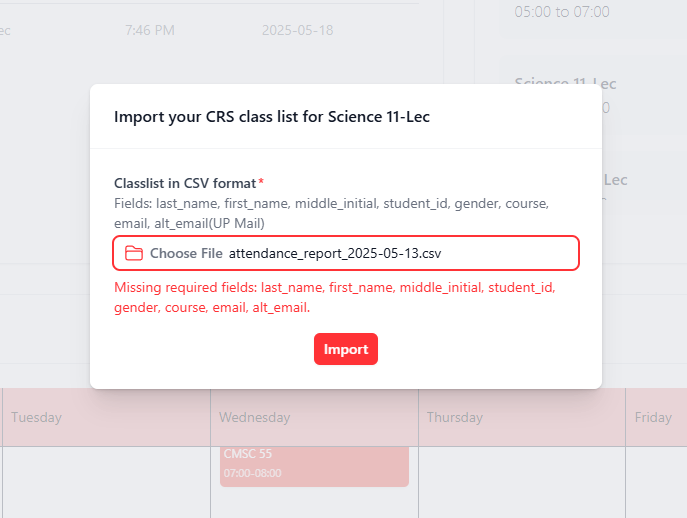
\includegraphics[width=0.8\textwidth]{figures/chapter4/faculty_import.png} % Adjust width as needed
	\caption{Faculty Import using CSV}
	\label{fig:faculty_import}
\end{figure}
\begin{figure}[h] % 'h' places the figure approximately here in the text
	\centering
	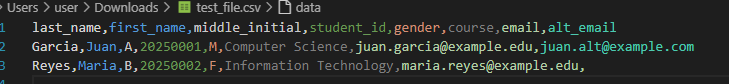
\includegraphics[width=0.8\textwidth]{figures/chapter4/faculty_import_csv.png} % Adjust width as needed
	\caption{CSV sample file}
	\label{fig:faculty_import_csv}
\end{figure}
\begin{figure}[h] % 'h' places the figure approximately here in the text
	\centering
	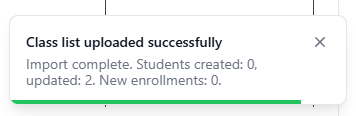
\includegraphics[width=0.8\textwidth]{figures/chapter4/faculty_import_success.png} % Adjust width as needed
	\caption{Import success}
	\label{fig:faculty_import_success}
\end{figure}
\clearpage
\subsection{Students CRUD operations}
By default, the \url{/students} tab will list all students under the logged in teacher.
\begin{figure}[h] % 'h' places the figure approximately here in the text
	\centering
	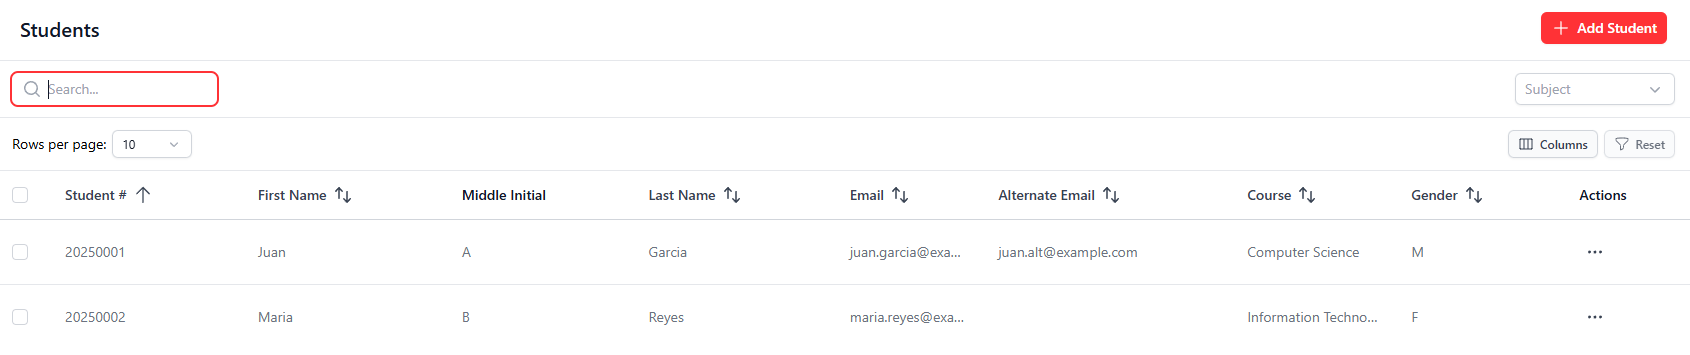
\includegraphics[width=1\textwidth]{figures/chapter4/student_list.png} % Adjust width as needed
	\caption{Students page}
	\label{fig:student_list}
\end{figure}
At this point, we still don't have information about the RFID of the student. We can add them by batch in this page. Connect the RFID scanner and scan the matching ID. The web app will wait for key events and automatically save the RFID of students scanned.
\begin{figure}[h] % 'h' places the figure approximately here in the text
	\centering
	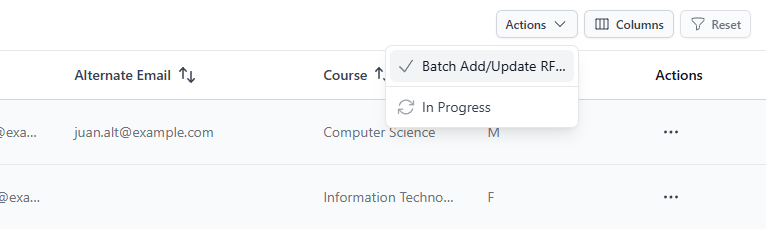
\includegraphics[width=1\textwidth]{figures/chapter4/batch_rfid.png} % Adjust width as needed
	\caption{Batch Actions}
	\label{fig:batch_rfid}
\end{figure}
\begin{figure}[h] % 'h' places the figure approximately here in the text
	\centering
	
\includegraphics[width=1\textwidth]{figures/chapter4/batch_rfid_scan.png} % Adjust width as needed
	\caption{Automatic scanner. The faculty do not need to press anything, as the scanner simulates an Enter press after scanning the RFID number.}
	\label{fig:batch_rfid_scan}
\end{figure}
\clearpage
\subsection{Web equivalent of the time-in and time-out process}
It also has a web equivalent of the PyQT5 time-in and time-out processing, albeit much slower. See Figures \ref{fig:faculty_import} and \ref{fig:frontend}.
\begin{figure}[h] % 'h' places the figure approximately here in the text
	\centering
	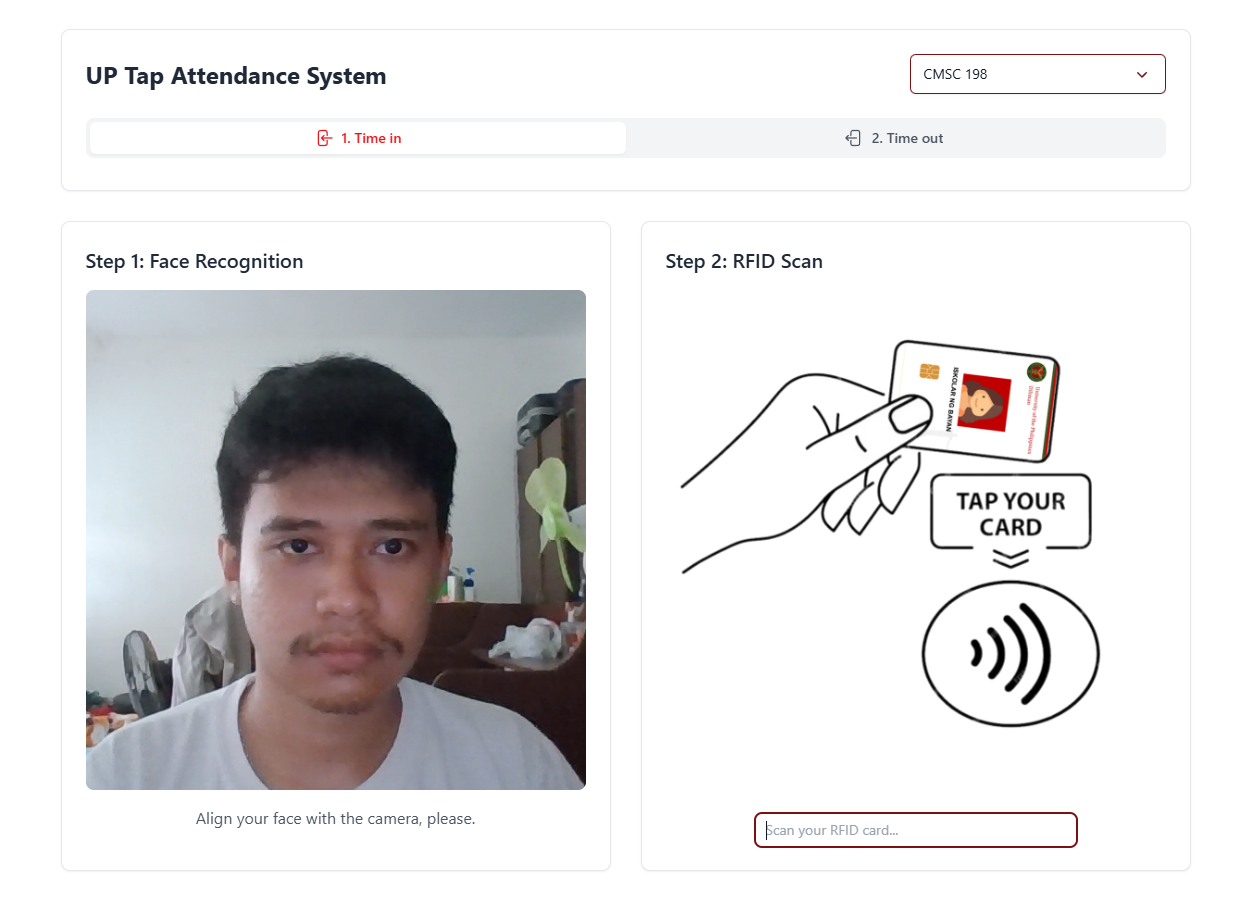
\includegraphics[width=1.0\textwidth]{figures/chapter4/frontend.png} % Adjust width as needed
	\caption{Time in and Time out Page}
	\label{fig:frontend}
\end{figure}

\begin{figure}[h] % 'h' places the figure approximately here in the text
	\centering
	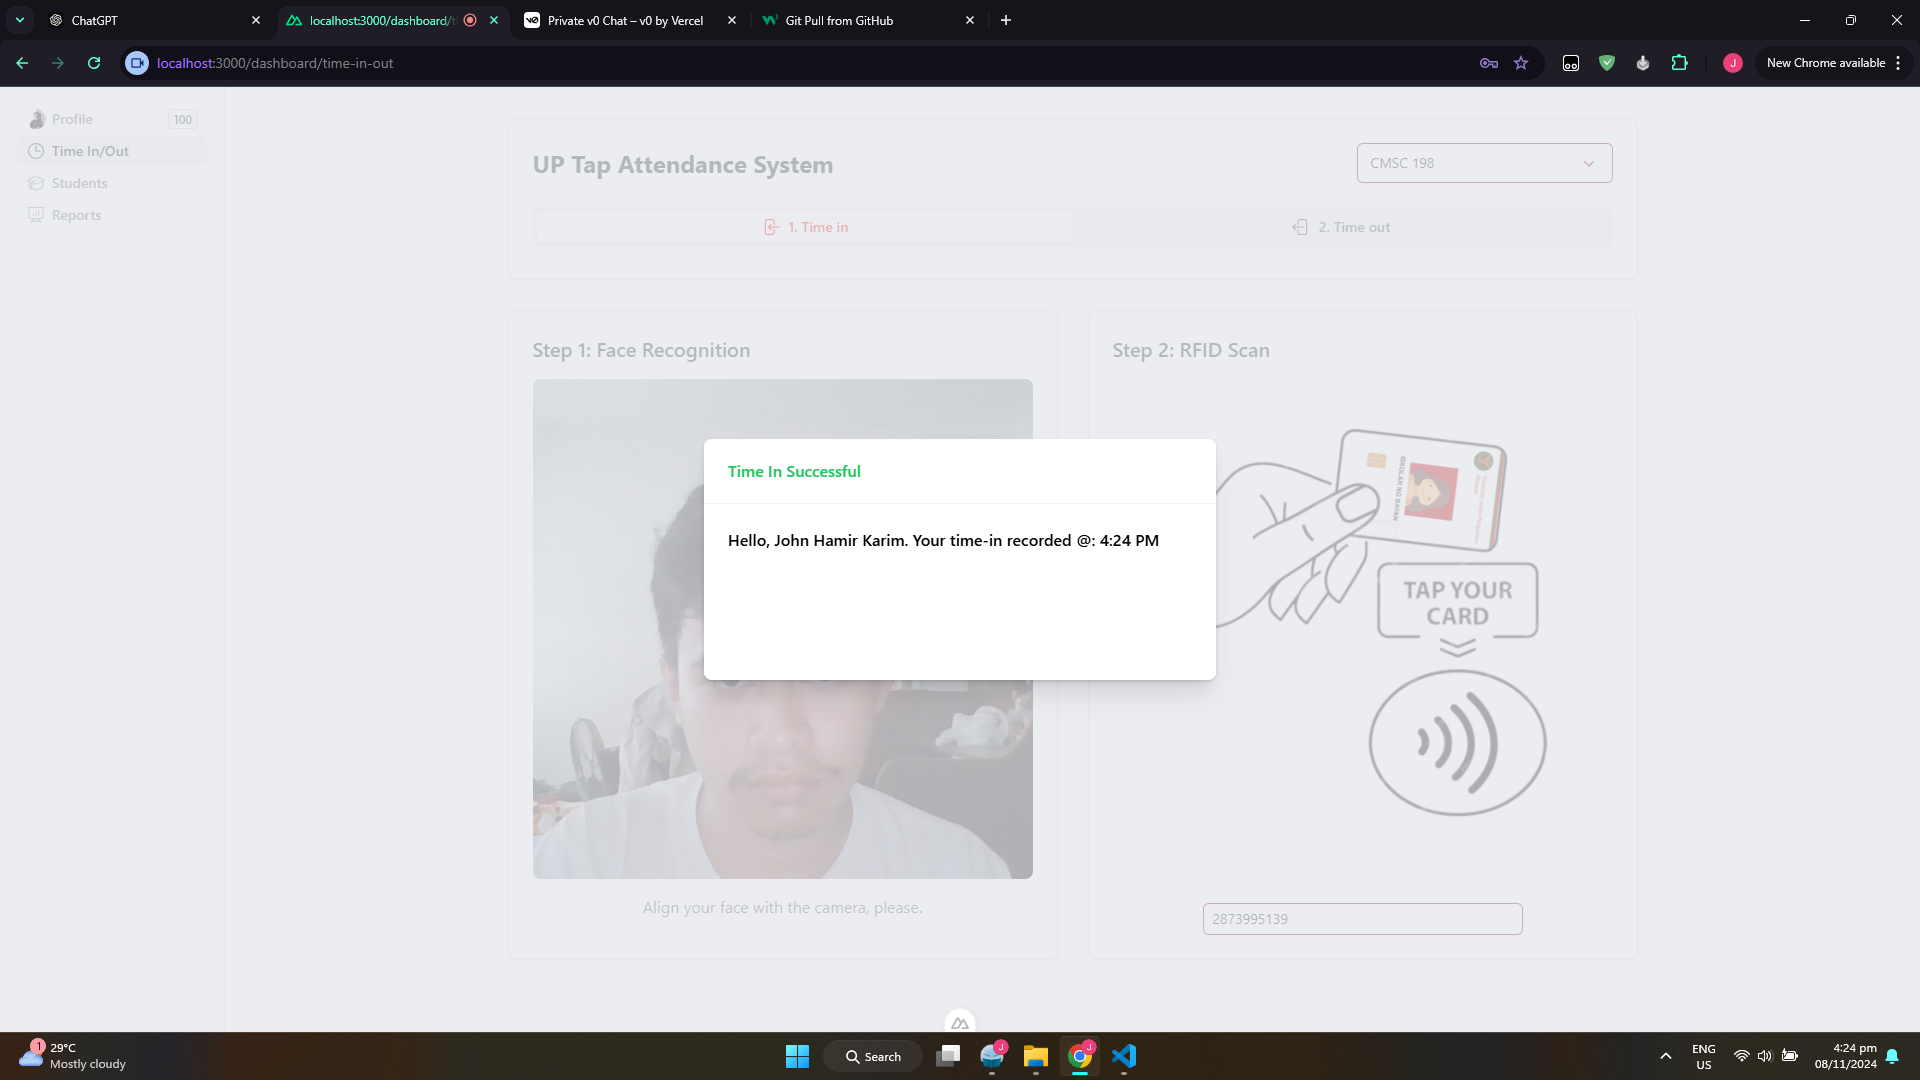
\includegraphics[width=1.0\textwidth]{figures/chapter4/success.png} % Adjust width as needed
	\caption{Successful Time In}
	\label{fig:success}
\end{figure}
\begin{figure}[h] % 'h' places the figure approximately here in the text
	\centering
	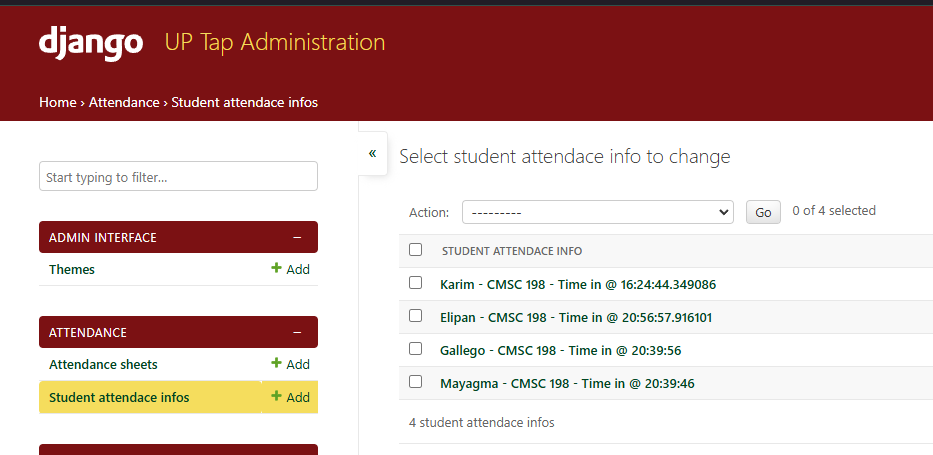
\includegraphics[width=0.75\textwidth]{figures/chapter4/backendrecord.png} % Adjust width as needed
	\caption{Django saving the attendance time instance in 24-hr format}
	\label{fig:record}
\end{figure}

\clearpage
\section{MobileFacenet in detail}
The MobileFacenet model for was used face verification. The model takes in a 112x112x3 image and outputs an embedding(a mathematical representation of face). We then use Cosine similarity with a certain threshold to compute if two embeddings are similar, therefore concluding that both identities are the same. The model was converted to a Tensorflowlite model to run faster on the Raspberry Pi 5 hardware. The final size of the model is 863Kb.

\subsection{Model Architecture}
Figure \ref{fig:mfn_arch} Shows the general architecture of the model as defined in the MobileFacenet paper \cite{chen2018mobilefacenets}.
\begin{figure}[h] % 'h' places the figure approximately here in the text
	\centering
	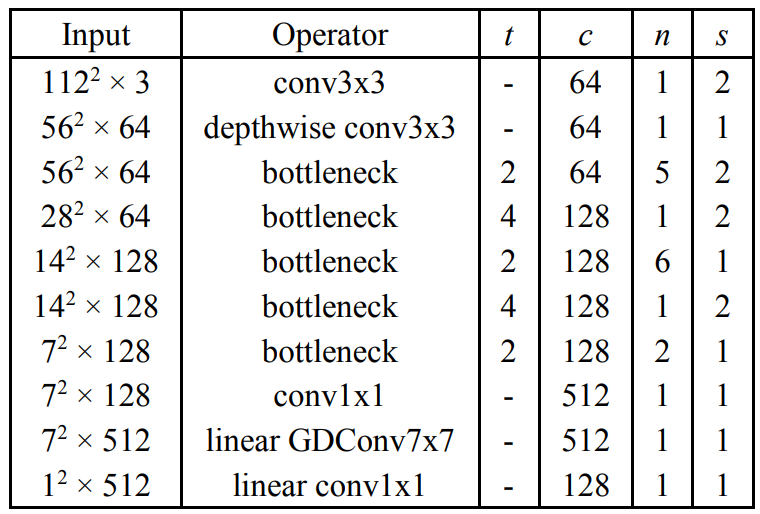
\includegraphics[width=0.5\textwidth]{figures/chapter4/mfn_arch.png} % Adjust width as needed
	\caption{MobileFaceNet}
	\label{fig:mfn_arch}
\end{figure}

\clearpage 
\subsection{Metrics}
We tested the accuracy of the model using the Labeled Faces in the Wild (LFW) Dataset via sklearn. The dataset includes 13,233 images of 5,749 people. The sklearn package provides a 300 pairs of same + 300 pairs of different people per fold. We tested the model in 10 folds.
Compared to models of hundreds of MB in size, the performance of the model is good but can be better. An AUC of 0.77 means that if we pick one genuine (same‐person) pair and one impostor (different‐person) pair at random, there’s a 77\% chance the model will score the genuine pair higher.
\begin{figure}[h] % 'h' places the figure approximately here in the text
	\centering
	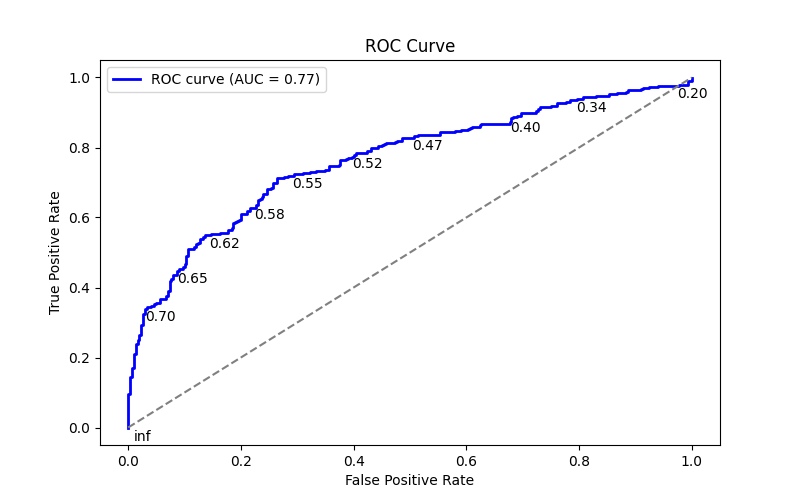
\includegraphics[width=1\textwidth]{figures/chapter4/roc_curve.png} % Adjust width as needed
	\caption{ROC AUC}
	\label{fig:roc_curve}
\end{figure}

\clearpage
Next we check the overall accuracy at the chosen threshold. We chose the 0.6 as threshold for a good balance of security and reliability. The threshold posted an average accuracy score of 68.6\% on all ten folds. While not impressive, note that the model we test here is a TensorFlow Lite version which was compressed for faster inference on RPI 5.
\begin{figure}[h] % 'h' places the figure approximately here in the text
	\centering
	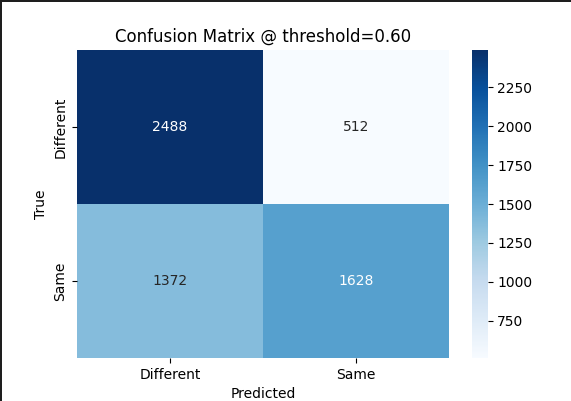
\includegraphics[width=0.75\textwidth]{figures/chapter4/fixed_thresh_matrix.png} % Adjust width as needed
	\caption{ROC AUC}
	\label{fig:fixed_thresh}
\end{figure}



\section{YoloV8n for Face Detection}
We used a pretrained YoloV8n model for face detection by Arnab Dhar on Huggingface. The main motivation was because Yolo models were the first to officially support exporting and deploying a model to the Raspberry Pi AI Camera. The Ultralytics team abstracted the process of model quantization and compression using Sony's Model Compression Toolkit into their Python library. Compression and quantization was required as the IMX500 chip has a limited memory for inference at approximately 8mb only. The original pickle file is around 6.0mb which is compressed down to around 3mb per Ultralytics documentation. It can be further finetuned using personal dataset for better accuracy. 





